
\chapter{Conclusions}\label{conclusions}

All variants of \textsf{RPHash} share a number of similar performance advantages over other traditional
methods while also suffering similar drawbacks.  Subsequent attempts to mitigate these drawbacks
resulted in the various version of \textsf{RPHash} and configurations.  In this section we discuss those
common attributes as well as a breakdown of the variant specific attributes and how they compare to
other clustering algorithms.

\section{Clustering Performance}

In this section we discuss how \textsf{RPHash} clustering performance compares to classic and state-of-the art
clustering algorithms.  While the primary goal of clustering is ill-posed, performing well on an
ensemble of clustering metrics is generally regarded as an overall useful measure of clustering
performance.

\subsection{RPHash}

Table \ref{compareOtherAlgo} gives an exhaustive comparison of the standard \textsf{RPHash} algorithm to
various other common clustering methods.  In this section we focus only on the listed clustering
performance.  Regarding clustering performance, we report measures for \emph{adjusted rand index}
and \emph{cluster purity}.  \textsf{RPHash}'s performance is highly dependent upon the dataset being
clustered.  In general it performs better than most of the agglomerative methods for all datasets.
The exception for agglomerative methods is the Ward's Linkage, which performs better in some of the
chosen datasets.  This performance often echoes that of $k$-means performance, on the same
datasets.  While $k$-means tends to outperform \textsf{RPHash} in regard to overall performance, none of the
performances are better by a significantly large margin.  SOTA seems to perform most similarly to
\textsf{RPHash}, with similar ARI and Purities for all datasets.  The overall goal however is not that \textsf{RPHash}
outperforms other metrics in terms of clustering performance, rather that it is comparable, with the
an advantage in processing speed.  We investigate this further in Section \ref{rptiming}.

Table \ref{localWinners} gives more detailed performance for an optimized configuration of \textsf{RPHash}
against $k$-Means.  As before, \textsf{RPHash} and $k$-Means alternate between best performance, with only
minor deviations between the two.  The reconfigurability of \textsf{RPHash} is important in this case because
it can be optimized for the particular dataset, while $k$-means is less flexible in configuration.

\subsection{Streaming RPHash}

The performance of \textsf{streamingRPHash} is shown in Figure \ref{indoor-measures} and
Figure \ref{human-measures} as a function of streamed batches of data.  On both datasets
\textsf{streamingRPHash} tends to find a good local minima for the Within-Cluster Sum of Squared
Error metrics.  However, \textsf{streamingRPHash} tends to suffer on some external metrics such as
the adjusted rand index, and internal metrics that tend to favor cluster separability, such as Dunn
Index and Silhouette Index.  Further analysis of these results show a bias in
\textsf{streamingRPHash} that suggests it favors solutions to the facility location problem over the
more general clustering problem.  This may be exacerbated by the fact that \textsf{streamingRPHash}
does not specifically label noise or outlier vectors, which can result in poorer values pertaining
to Silhouette Index and Dunn Index.  This is mainly due to noise clusters skewing the inter/intra
-cluster distance ratio.

The performance of \textsf{streamingRPHash} on synthetic datasets with varying dimensions is shown in
Figure \ref{scalability-measures}.  For synthetic datasets \textsf{streamingRPHash} does quite well,
matching the optimal performance of the best stream clustering algorithms. In all cases it
outperforms Streaming $k$-Means and Damped Sliding Window.

The scalability of \textsf{streamingRPHash} for Runtime and memory is shown in Figure
\ref{scalability-perf}.  As expected the resource requirements of \textsf{streamingRPHash} and
streaming $k$-means are substantially lower than those of other tested algorithms.  This advantage
becomes increasingly significant as the dimensionality of the input vectors grows.  Although
streaming $k$-means maintains a consistently better bound on both memory and processing time, the
overall growth complexity is similar, which suggests optimizations to \textsf{streamingRPHash} could
put it in reach or streaming $k$-means' performance.

The noise study demonstrates an addition benefit of \textsf{streamingRPHash}.  As expected, a
gradual decrease in clustering accuracy of all algorithms is observed as the amount of noise
increases in the data stream.  However, there are some interesting patterns in clustering results
produced by \textsf{streamingRPHash}.  Its clustering accuracy clearly exceeds that of other
algorithms in the presence of 2\% noise.  As the amount of noise begins to increase in the data
stream, Damped Sliding Window and Biased Reservoir Sampling seem to produce better clustering in
terms of external measures.  However, even with the increasing noise, \textsf{streamingRPHash}
continues to give the best clustering results in terms of internal measures.  In particular, its
WCSSE values remain the lowest, and sometimes lower than baseline values, even in the presence of
noise as high as 60\% and 75\%.  This can be explained if we look into how labels are assigned to
random noise points at the time of data stream generation.  As mentioned before, each noise point is
assigned to a cluster whose centroid is the closest to that noise point.  Thus, a noise point, which
is assigned to a cluster $i$, may actually be closer to the boundary of another cluster $j$.
Therefore, it is possible that a clustering algorithm places a noise point in a \emph{more
  appropriate} cluster than the data stream generator does.  In other words, the clustering
algorithm may be able to find better centroids to incorporate noise points, thus producing more
compact clusters than ground-truth partitions.  In this case, the clustering algorithm will produce
better values of internal measures than the baseline values.  On the other hand, since external
measures try to capture the agreement between ground-truth partitions and clusters detected by an
algorithm, the values of external measures will clearly remain low.  This is why
\textsf{streamingRPHash}, when applied on noisy data streams, performs much better in terms of
internal measures.  The apparent decrease in values of external measures is merely due to the
disagreement with ground-truth labels of noise points.

To summarize our findings from the scalability study: we discover a major strength of
\textsf{streamingRPHash} and conclude that the algorithm is capable of producing perfect clustering
when the data stream consists of a mixture of Gaussian distributions without any noise.  For real
world, and data containing a significant amount of noise, it may be useful to augment
\textsf{streamingRPHash} with the ability to label observations as noise.

\subsection{Tree Walk RPHash}

On real world and synthetic datasets, the Tree-walk RPHash algorithm tends to perform better than
the standard \textsf{RPHash} and \textsf{streamingRPHash} algorithms.  In contrast the Adaptive LSH algorithm
in both the Streaming and Standard \textsf{RPHash} algorithm has a slightly mixed result.

In Figure \ref{twrpvothers} we see that standard \textsf{RPHash} and the Leech decoder outperforms the
adaptive LSH algorithm and the \textsf{TWRP} algorithm.  While this result is in opposition of our claim that
the \textsf{TWRP} is best among \textsf{RPHash} variants, it is important to note that the experiment was performed on
a highly synthetic dataset with no noise, and tightly clusterable data.  The test in fact is very
similar to the results in Figure \ref{bbvar} where the Leech Lattice decoder was well suited to
finding tight, uniform clusters scaled between -1 and 1.  It is not until we look at more
realistically generated datasets and robust clustering metrics that we see the advantage of \textsf{TWRP}.
Figures \ref{perfdim1}, \ref{perfdim2}, and \ref{perfdim3} show \textsf{TWRP} performing optimally for all
datasets at all dimensions, while the standard \textsf{RPHash} algorithm and $k$-Means show considerable
variance in Purity, ARI, and WCSSE.  In Figure \ref{w2vwcss} and Figure \ref{w2vratio} we look at the raw
WCSSE scores, and the ratio of WCSSE for \textsf{TWRP} and the $k$-Means++ algorithm on 1000 dimensional,
real world, Word2Vec data.  Overall, \textsf{TWRP} performs within $5.1\%$ of $k$-Means++.  This is significant
if we consider the scalability difference between \textsf{TWRP} and $k$-Means++.  Figure \ref{w2vproctime}
shows these differences, and while $k$-Means++ seems to grow quadratically with the number of
clusters, \textsf{TWRP} remains constant.  This is significant, because \textsf{TWRP} could potentially output any
number of micro-clusters to some, more robust machine learning algorithm, with no change in
processing time requirement.

\section{Noise Resilience}

All variants of the \textsf{RPHash} algorithms are noise robust.  This is primarily due to the density mode
search common in all algorithms, ignoring data that resides outside the partition region.  In Figure
\ref{noise-measures} we show the performance of \textsf{streamingRPHash} in regard to injected noise.  In
regard to WCSSE, \textsf{streamingRPHash}s outperforms all other clustering algorithms on noise resilience.  While among
other performance metrics, it tends to be in the top three.  Standard \textsf{RPHash} and \textsf{TWRP} are compared
in Figures \ref{noiseacc2}, \ref{noiseacc2} and \ref{noiseacc2} on ARI, Purity and WCSSE as a function of
injected noise.  For ARI and Purity, \textsf{TWRP} outperforms standard \textsf{RPHash} and the other comparison
algorithms up until the highest levels of injected noise $>35\%$.  Standard \textsf{RPHash} outperforms \textsf{TWRP}
on WCSSE metrics, but not by a very large margin.

\section{Timing Results}

A principal focus and motivation for this work, is to reduce the time and overall complexity of
current clustering methods.  As expected, \textsf{RPHash} and its variants outperform all other tested
clustering methods on processing speed and asymptotic complexity.  Time results at linear with
smaller constant factors than many other clustering methods.

\subsection{RPHash}\label{rptiming}

In Table \ref{compareOtherAlgo} we see that the standard \textsf{RPHash} algorithm often bests comparable
clustering algorithms by at times orders of magnitude on larger datasets.  Furthermore the growing
deviation between processing times in regard to dataset sizes suggests and overall asymptotic
complexity difference over other tested algorithms, which is verified in the previous sections
runtime analysis.  While agglomerative methods and SOTA tend to require considerably more time to
process than \textsf{RPHash}, $k$-Means is sometimes regarded as a near linear runtime algorithm
($\theta(loglog(n)*n)$).  However in a direct comparison shown in Table \ref{localWinners} we can
see that \textsf{RPHash} outperforms $k$-Means considerably on runtime.  This suggests that while $k$-Means may
have near linear asymptotic complexity, it exhibits considerable constant factor offsets.

\subsection{Streaming RPHash}

Similar to standard \textsf{RPHash}, \textsf{streamingRPHash} performs well on runtime.  While standard
\textsf{RPHash} was not compared against streaming $k$-Means, \textsf{streamingRPHash} was.  Streaming $k$-Means
in Figure \ref{indoor-measures} and Figure \ref{human-measures} outperforms \textsf{streamingRPHash} on
runtime.  However both algorithms exhibit similar scalability, as suggest by Figure
\ref{scalability-perf}.  It is likely that these performance differences could be overcome with
minor implementation optimization.

\subsection{TWRP}

The scalability with respect to dimension of \textsf{TWRP} and standard \textsf{RPHash} is shown in Figure
\ref{twrp_scale}.  In the plot we see that there is no contest between the \textsf{RPHash} algorithms and the
comparison algorithms SOTA and $k$-Means.  While the Table \ref{scalability} shows an even more
dramatic difference between both versions of \textsf{RPHash} and the agglomerative algorithms.  \textsf{TWRP} is
almost 688 and 4795 times faster than $k$-means and agglomerative hierarchical respectively for the
noise datasets having dimensions 10000x6500. We can see the growth of time as the dimension
increases in Figure \ref{twrp_scale} . RPhash and \textsf{TWRP} has almost no growth when compared to the
other algorithms.

Figure \ref{w2vproctime}, Table \ref{scalability} and Table \ref{perftimetable} provide similar evidence
regarding the superiority or \textsf{RPHash} algorithms in general
With the complexity growth of \textsf{RPHash} being nearly linear, with small constant factor offsets.
Therefore we can see that one of the biggest advantages of \textsf{RPHash} is that it achieves such
comparable clustering accuracy with minimal costs of runtime . This makes \textsf{RPHash} suitable for
applications where the dimension or volume of data is very high.

\section{Parallelism}

A primary focus of the \textsf{RPHash} algorithms is to enable naive parallelism through the coordination of
generative mathematical functions and approximate data sketches, instead of costly verbose
interprocess communication.  The results in Figure \ref{minskispeedup} show that our assumptions about
\textsf{RPHash} parallelism, are to some degree, correct.  For data centric algorithms like \textsf{RPHash}, the ratio
of parallel to sequential code, per Amdahl's law, is strongly dictated by the input data size.
However to not bias our parallelism with the input IO of our test machine's memory subsystem, all
parallel experiments were done on in memory datasets, resulting in a limit to the overall amount of
achievable parallelism.  It is our belief that larger datasets may show further advantages for
\textsf{RPHash} in regard to parallel speedup.

Standard \textsf{RPHash} appears to enjoy the greatest advantage in regard to parallel speedup. The results
for \textsf{RPHash} were edited to remove, outlier data points in which memory contention for many nodes,
caused errors as parallelism grew.  This is more an artifact of our chosen method of parallelism,
than that of an intrinsic algorithm design.  Namely, standard \textsf{RPHash} tends to use significantly more
memory per core than our sketch based algorithms.  This Memory requirement presented itself when
scaling to more processing nodes, and caused a memory bottleneck around 15 nodes.  Fifteen nodes
however is a reasonable baseline to establish the predictable parallelism.  For the intended
distributed implementation of \textsf{RPHash} in MapReduce or Spark, it is unlikely these physical memory
restrictions would exist.

Interestingly, \textsf{TWRP} which would presumable be sequentially bound by the off-line Tree walk procedure
and per vector, shared sketch update step, actually parallelizes quite well.  The likely reason for
this is that the off-line step does not contribute significantly to the overall number of
computations required for both on-line and off-line processing steps.  Furthermore, the shared memory
environment of our experimental setup, allows for fast access to the Count-Min Cut Tree structure.
In the distributed setting, this would not be the case.  However, due to the additive nature of the
Count-Min Sketch, completely independent update of the Count-Min sketch would be trivial and would
only require a $\theta(log(N))$ number of steps to reduce the $N$ sketches.

\textsf{streamingRPHash} suffered a poorer than expected speedup performance.
\textsf{streamingRPHash} utilized vector parallelism, in which processing nodes were scheduled by a
master node, to the first available thread.  This naturally results in a sequential bottleneck at
the master node.  However, it additionally stresses cache prediction, in real world CPUs, due to our
greedy vector-to-CPU assignment.  The greedy assignments are strongly influenced by the chosen LSH
algorithm, which in this experiment was the Leech Decoder, which is determined by the randomly
generated data vectors.  This cache pressure along with the sequential bottleneck, make
\textsf{streamingRPHash} a poor candidate for shared memory system parallelization.  However, for
distributed systems in which vectors are fetched from a remote source, the parallelism should only
be bound by the intermittent off-line steps.  In contrast, both \textsf{TWRP} and standard \textsf{RPHash} were able to
partition the problem equally among processing nodes and then work on the sets of vectors
independently.

An alternate hypothesis however, is that our results may be somewhat under represented due to our
test system only having 16 physical cores and 32 threads due to Hyper-Threading, instead of 32
truly independent processing nodes.  Hyper-Threading is a technology that effectively shares the
resources of a single processing pipeline, between two processing workloads, with the assumption
that underutilized processing sub-units will achieve better overall utilization.  This however is not
completely equivalent to two independent processing units.  The saturation of one unit, such as the
Floating Point sub processing unit, could cause a bottleneck.  Furthermore, hyper-threading is also
bound by there only being one physical, memory management unit per core, which could be a source of
further IO saturation.  Another likely candidate for our sub-linear speedup performance could be our
test system's Quick Path Memory controller, resulting in non-uniform memory data access patterns.
Attempts were made to optimize this access pattern through both the Java NUMA flag, and the
operating system `numactl' meta-processing environment.  Both alterations failed to achieve
significantly different results (timing was worse on all tests).  These possibilities further
suggest that a completely independent distributed processing environment may achieve better overall
parallelism.

\section{Overall Conclusion}

The \textsf{RPHash} algorithms combines approximate and randomized methods in a new way to solve
issues of scalability and data security for cluster analysis on distributed data.  The runtime and
clustering performance of our \textsf{RPHash} algorithms are similar to that of the standard $k$-means
clustering algorithm, with the added benefit of being scalable to very large datasets.  This
randomized, clustering algorithm is well suited for ill-posed, combinatorially restrictive problems
such as clustering and partitioning.  This assertion is complemented by a similar inversion
regarding clustering and computing, in which real world problems tend to converge much faster than
adversarially crafted worse-case problems.

The principle assumption in this work is that approximate and exact clustering, are qualitatively
similar due to noise, redundancy, data loss, and the curse of dimensionality.  Furthermore, the
addition of random noise to the clustering dataset resulting from the random subspace projection
requirement, provides some degree of non-deterministic process, so subsequent iterations of the
algorithm could potentially find better results.  Making the process of finding better clustering
results, a matter of available processing time and resources.  Furthermore, the destructive
projection process affords us a certain degree of data privacy while requiring no additional
processing.

\subsection{RPHash Conclusions}

The \textsf{RPHash} algorithm offers a fast highly scalable algorithm for data clustering that shows
potential for distributed computing that can benefit well from addition processing resources, and is
secure.  \textsf{RPHash}'s simple straightforward structure results in a predictable time requirement.  The
processing time predictability is beneficial for time dependent cases where completion time is more
important than minor errors in clustering accuracy.  Overall, \textsf{RPHash} is much faster than other
clustering algorithms.  Some drawbacks of the standard \textsf{RPHash} algorithm, is that the results can be
order dependent, and sometimes unstable.  Multiple runs can fix some of these issues, but the
overall stability may be an outstanding problem, that we suggest \textsf{TWRP} remedies.

\subsection{Streaming RPHash Conclusion}

\textsf{streamingRPHash} Is a fast accurate single pass clustering method for high dimensional data
streams.  The growing number of massive, high dimensional streaming data sources can take advantage
of the benefits of quick, accurate, scalable and distributed processing of \textsf{streamingRPHash}.
We show that our method is faster than most of our comparative streaming clustering algorithms. 
while performance is underwhelming on the HAR dataset, \textsf{streamingRPHash} does quite well on
the UJII dataset.  The deviation in performance between datasets suggests that
\textsf{streamingRPHash} may not be well suited for all datasets.  However, when data is well
behaved, containing predominantly spherical clusters in high dimensional space,
\textsf{streamingRPHash} outperforms all other streaming clustering methods.  This may be a result
of the sub-space projection, being well equipped to capture the overall data variance for these types
of datasets.  Another feature of \textsf{streamingRPHash} is that it is robust to noise,
outperforming all other clustering algorithms on clustering metrics.  These benefits however are
overshadowed by \textsf{streamingRPHash} processing efficiency, scalability and memory usage.
\textsf{streamingRPHash} compares well to Streaming $k$-means in timing and memory usage.  While
shared memory parallelism is below our expectations, the potential for distributed processing, is
positive, and would likely exceed the scalability of streaming $k$-means which incurs a sequential
bottleneck when checking and updating a shared list of nearest cluster centroids.

\subsection{TWRP Conclusions}

In this work we introduced the Tree-Walk Random Projection (\textsf{TWRP}) clustering technique for
clustering large datasets with log-linear processing complexity.  We applied our clustering
technique on real and synthetic data of varying noise levels.  Our method performed comparable to
various other common clustering methods, while improving significantly upon the overall required
processing time.  \textsf{TWRP} improves upon standard \textsf{RPHash} clustering performance and in many cases
performs better than $k$-means and similarly to Ward's Linkage hierarchical agglomerative
clustering.  Importantly, it does so, while achieving a similar processing time requirement and
scalability as standard \textsf{RPHash}.  Furthermore the \textsf{TWRP} algorithm improves upon \textsf{RPHash}'s already
relatively good noise suppression performance.  \textsf{TWRP} also improves upon \textsf{RPHash} by offering more
stable results between runs, that border on deterministic behavior.  Another advantage of \textsf{TWRP} is
that is shows strong potential for shared memory and distributed parallelism.  In addition, \textsf{TWRP} is
also amenable to streaming environments, due to its base structure being the Count-Min Cut-Tree.
The Count-Min Cut-Tree is an error bounded constant memory sketch, that succinctly encodes the
required data structure of the off-line clustering process.

\subsection{Code Repository}
The \textsf{RPHash} Java source code is released under an open source license and is freely
available at \url{github.com/wilseypa/rphash-java}.  Python versions of \textsf{TWRP} are available on-line at
\url{https://github.com/leecarraher/PyRecRPHash}.  Plots and figures are available by request
\url{mailto://leecarraher@gmail.com}

\section{Future Research}\label{further}
In this section we give suggestions for potential future research following the \textsf{RPHash} clustering framework.  We discuss
a further distributed framework for \textsf{streamingRPHash}, and \textsf{RPHash} as a pre-clustering technique for more robust
clustering methods like topological data analysis(TDA).
We also suggest more practical implementation improvements like GPU processing. Lastly we discuss the potential of the 
general Count-Min Cut Tree as a general space partitioning sketch.

\section{Spark Implementation}

\begin{figure}
    \centerline{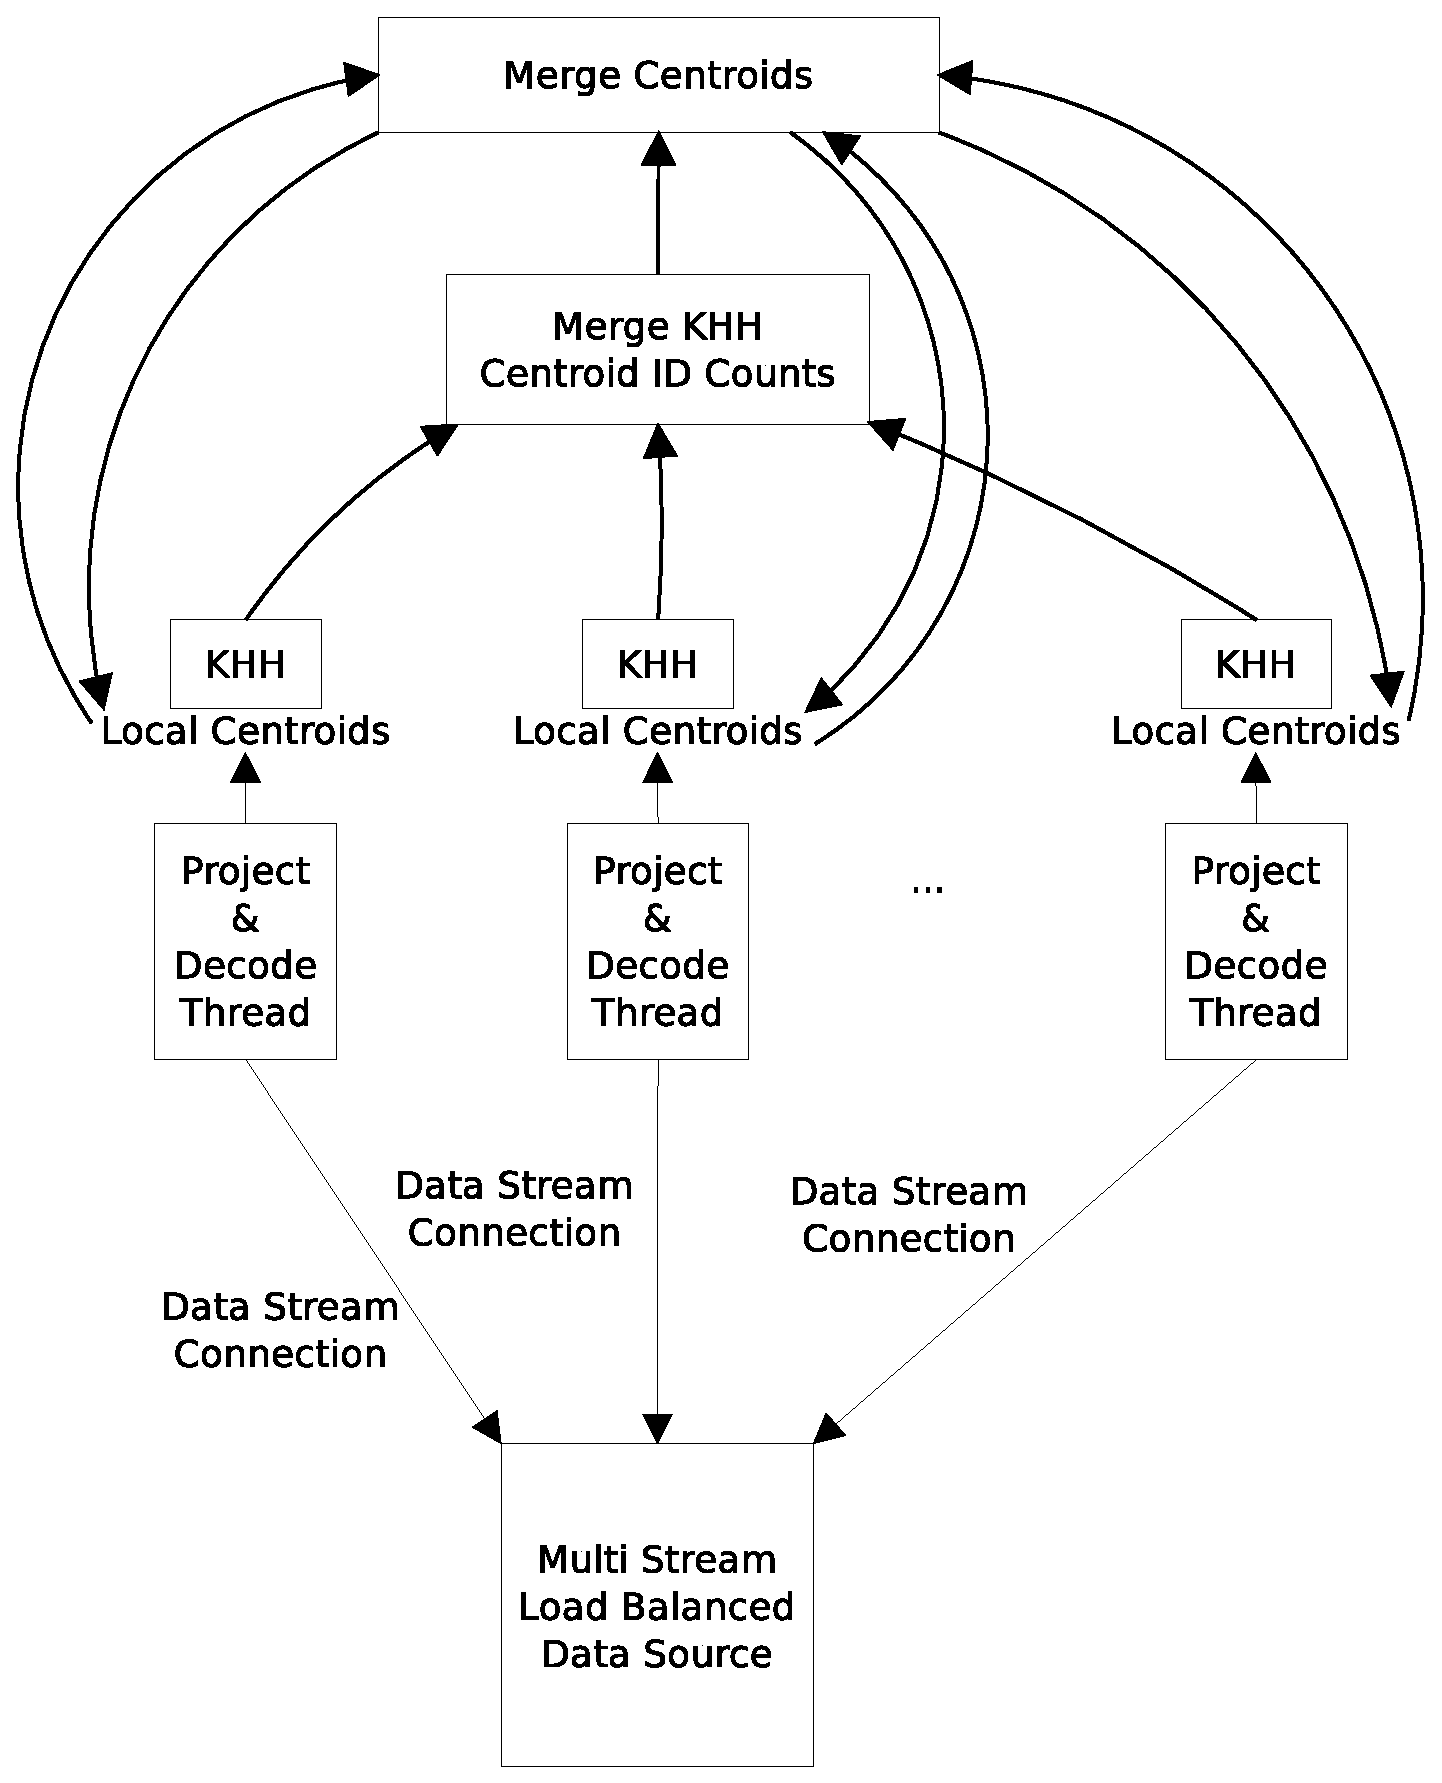
\includegraphics[width=.7\textwidth]{figs/sparkrp}}
    \caption{Spark Streaming RPHash Diagram}\label{sparkrp}
\end{figure}

Spark is a distributed computing framework loosely based on functional parallelism that runs on
Hadoop and other similar frameworks.  Spark is similar in design to MapReduce functional dissection
for parallel algorithms, however, unlike the standard Hadoop MapReduce algorithm, it is geared toward
multi-pass processing common in machine learning algorithms, by leveraging RAM caching of persistent
states between Map and Reduce phases.  Furthermore, Spark allows for streaming interfaces for
parallel processing, capable of extending the \textsf{streamingRPHash} algorithm.  A future direction
for \textsf{streamingRPHash} would be to utilize the input stream methods in spark, to implement 
\textsf{streamingRPHash} as a fully distributed stream based clustering method.  The implementation could read
streams independently from disconnected data streams, building independent data structures, and merging the 
results when requested.  Similar to the \textsf{streamingRPHash} diagram given in Figure \ref{rphash}, we give a 
distributed extension in Figure \ref{sparkrp}. 

\subsection{Topological Data Analysis}

An interesting emerging field in machine learning is topological data analysis(TDA). TDA attempts to
overcome some of the issues inherent with orthogonal metric data embeddings by regarding not just
the data, but the connectivity between the data.  Somewhat similar to manifold learning methods, in
which data is regarded as being embedded in some complex manifold, TDA goes further, by removing the
restriction that a surface be locally differentiable. In this way, surfaces can have holes, and true
discontinuities.

While TDA work is still emerging, there is a significant gap between theoretical understanding and
practical application.  In particular, many TDA algorithms are graph based and therefore,
combinatorially bound.  However, by using the concept of micro-clusters, arbitrarily available through
\textsf{RPHash} clustering, with no computation penalties, one could potentially reduce the complexity of
TDA algorithms, to these representative micro-clusters, followed by subsequent refinements. 

\section{GPU Leech}

Previous work \cite{carraher} on a graphics processing unit (GPU) implementation of the Leech Decoder for LSH could readily be
used to accelerate the \textsf{RPHash} algorithm.  While performance monitoring showed the principal
occupation of \textsf{RPHash} was in the projection step, accelerating just the LSH may only result in a
small speedup.   However, if we were to combine both the projection and a GPU based implementation of
LSH, we may be able to take advantage of GPU memory locality, and achieve considerably high GPU core
occupancy (a principle measure for GPU parallelism).

\subsection{Bounded Error Compressed Cut Tree}


While the results from Tree Walk Random Projection Hash are promising, a more interesting data
structure is defined that may have application beyond cluster analysis. In particular, this structure,
which will be referred to as a \emph{Bounded Error Compressed Cut Tree} has the potential of 
accelerating and making feasible a variety of interesting learning and data space exploration problems. 

We briefly review its structure here.  In \textsf{TWRP} we partitioned a data set by a sequence of orthogonal
vectors corresponding to the origin of each subsequent dimension.  This partitioning results in a 
$d$ length LSH encoding for every vector.  The hashes are then stored as a compressed representation
in the Count-Min Sketch.  As an aside, while we make the restriction that all hyperplanes intersect the origin,
BECC-Trees could also be composed of any set of hyperplanes rotated any number of times.  This
structure which we treat as a vector density oracle for \textsf{TWRP} clustering could be used similarly, for a variety
of other purposed. The basic setup would involve changing either the tree traversals method, or by storing some 
alternative metric in the nodes.  The tree, again never being fully realized, uses the Count-Min Sketch as an
 approximate partitioning oracle.  Therefore any tree based solution to a graph problem in which a
cut oracle would be helpful, could be solved in $1\over \epsilon$ space.

The true power of this structure comes 
of course comes from the parameterization of the Count-Min Sketch, which allows one to set the level of 
acceptable error, for tree based oracle problem.  The Count-Min Sketch constrained to elements in a tree
can compress any exponentially large space partitioning problem, and is certainly worth further investigation.  
Our Bounded error compressed cut trees certainly demonstrate this property for clustering.  In addition, the ability 
of BECC Trees to consume a potentially unbounded data stream, and store only a sketch of its current structure to 
later be scrutinized and reconstruction is potentially applicable to off-line data stream inquiry.  

%The \textsf{streamingRPHash} algorithm combines approximate and randomized methods in a
%new way to solve issues of scalability and data security for cluster analysis of data
%streams.  The runtime and Precision-Recall performance of \textsf{streamingRPHash} is
%similar to that of the standard KMeans clustering algorithm, with the added benefit of
%being applicable to infinite data streams.  This randomized, clustering algorithm is well
%suited for ill-posed, combinatorially restrictive problems such as clustering and
%partitioning.  This assertion is complemented by a similar inversion regarding clustering
%and computing, in which real world problems tend to converge much faster than
%adversarially crafted worse-case problems.

%The principle assumption in this work is that approximate and exact clustering, are
%qualitatively similar due to noise, redundancy, data loss, and the curse of
%dimensionality.  Furthermore, the addition of random noise to the clustering dataset
%resulting from the random subspace projection requirement, provides some degree of
%non-deterministic process, so subsequent iterations of the algorithm could potentially
%find better results.  Making the process of finding better clustering results, a matter of
%available processing time and resources.

%Clustering has long been the standard method used for the analysis of labeled and
%unlabeled data.  Clusterings effects intrinsically identify dissimilar and similar objects
%in a dataset, often unattainable through standard statistical methods.  Single pass, data
%intensive statistical methods are often the primary workhorses for database processing of
%business logic and other domains, while clustering is often overlooked due to issue in its
%scalability.

%Applications such as Micro Array clustering, Protein-Protein interaction clustering,
%medical resource decision making, medical image processing, and clustering of
%epidemiological events all serve to benefit from larger dataset sizes that
%\textsf{streamingRPHash} enables.


\section*{Acknowledgments}

Support for this work was provided in part by the National Science Foundation under grant
ACI--1440420.


